\documentclass{report}

\usepackage[italian]{babel}
\usepackage[utf8]{inputenc}
\usepackage[hidelinks]{hyperref}
\usepackage{graphicx}
\usepackage[font=small,labelfont=bf]{caption}
\graphicspath{ {../assets/} }

\title{Report sul protocollo GREEN-WUP}
\author{Leonardo Emili}

\begin{document}
\maketitle
\tableofcontents

\chapter{GREEN-WUP}
\section{Il protocollo GREEN-WUP}

Il protocollo GREEN-WUP si inserisce nel contesto dei protocolli delle cosiddette \emph{green wireless sensor network} e pone tra i suoi principali
obbiettivi l'efficienza energetica dell'intera rete. Esso impiega le tecnologie di wake up radio, energy harvesting e semantic addressing. Il protocollo è
di tipo \emph{converge casting} ed è basato sull'assegnazione di hop count a ciascun nodo per poter distribuire i pacchetti dati
all'interno della rete.\\

Il protocollo è articolato in due fasi principali: in primo luogo avviene la fase di \emph{interest dissemination} dove si definisce la
topologia della rete da rispettare affinchè i nodi realizzino un corretto flusso di scambio dati; successivamente si assume che gli indirizzi di
wake up siano stati assegnati e si procede con lo scambio di dati che è governato da sequenze di wake up usate per risvegliare i nodi della rete. \\

Inizialmente il sink node avvia la fase di interest dissemination inviando
un primo \emph{command packet} che viene successivamente distribuito ai nodi sensori utilizzando l'algoritmo di \emph{flooding}.
L'obbiettivo di questo processo è di assegnare a ciascun nodo della rete un valore di hop count secondo un algoritmo iterativo: in particolare questo
avrà valore 0 nel solo caso del sink node, altrimenti $h$ se $h-1$ è il valore di hop count del nodo precedente. Al termine
di questa fase ciascun nodo sarà fornito un indirizzo di wake up $w=w_{h}w_{e}$ della lunghezza di 8 bit , dove il prefisso $w_{h}$ è definito dalla
codifica in 4 bit di $h$ e $w_{e}$ rappresenta la classe energetica del nodo, codificata nei restanti 4 bit. In particolare, l'energia di ciascun nodo viene
considerata relativamente all'energia rimamente nelle batterie e a quella derivata da sorgenti esterne. In definitiva, la codifica del suffisso $w_{e}$
viene calcolata a partire dalla discretizzazione in $k$ classi della disponibilità energetica di un nodo, dove $k$ rappresenta il numero delle classi
disponibili.\\

%image source: https://www.researchgate.net/figure/Topology-of-wireless-sensor-network-and-hop-count-of-sensors_fig7_285956270
\begin{figure}
    \begin{center}
        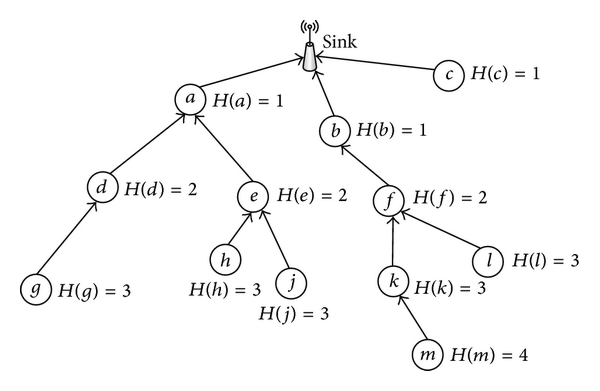
\includegraphics[scale=1.7]{hop-count-algorithm.png}
        \caption{Topologia della rete a seguito dell'assegnazione degli hop count}
    \end{center}
\end{figure}

A seguito della fase iniziale, ciascun nodo è in grado di calcolare il proprio indirizzo di wake up, che sarà periodicamente aggiornato in base alla loro
disponibilità energetica corrente. Questa idea realizza il principio del semantic addressing poiché in questo scenario
è possibile far riferimento ad un sottoinsieme di nodi della rete a partire dai loro valori di hop count e da quello della classe energetica.\\

A questo punto, se un nodo deve inviare un pacchetto dati può farlo seguendo una prima fase di selezione del nodo ricevente, seguita dal
successivo trasferimento del pacchetto dati, a seguito del quale verrà inviata una conferma per accertare l'avvenuta ricezione dello stesso. In particolare,
consideriamo un nodo $a$ non a diretto collegamento col sink node, con un valore di hop count $l$ ($l>1$). Al momento della richiesta di trasmissione dati,
$a$ prepara una sequenza di wake up $w$ con semantic addressing, scegliendo inizialmente la massima classe energetica $k$, e verifica facendo
\emph{carrier sensing} che il canale di comunicazione sia libero. Se il canale è libero allora procede inviando la sequenza di wake up che sveglierà tutti
e soli i nodi richiesti. Esso attende un contingente di tempo necessario affinchè i nodi destinatari, siano questi $B_1, B_2, \ldots B_n$ 
possano accendere le antenne principali (RX) ed invia in broadcast un pacchetto \emph{Request To Send} (RTS). Al momento della ricezione 
i nodi $B_1, B_2, \ldots B_n$ spengono la radio principale (SLEEP). Successivamente inviano al nodo $a$ una sequenza di wake up seguita da un pacchetto
\emph{Clear To Send} (CTS), utilizzando come indirizzo quello contenuto all'interno del pacchetto RTS precedentemente ricevuto, ed infine spengono
la radio principale (SLEEP). Si noti come venga ritardato l'invio del pacchetto CTS dai nodi utilizzando un tempo di \emph{jitter} randomico
per evitare collisioni. Al momento della ricezione del primo pacchetto CTS, $a$ seleziona il nodo che lo ha inviato, sia questo $B_i$,
per la ricezione del pacchetto dati. Quindi, $a$ verifica che il canale di comunicazione sia libero ed in caso positivo invia a $B_i$ una sequenza di wake up
seguita dal pacchetto dati. Dunque, $B_i$ ricevuto il pacchetto dati invia un \emph{acknowledgement packet} (ACK) ad $a$, va a dormire e prosegue la
ritrasmissione del pacchetto ricevuto sino ad arrivare al sink node. Infine, $a$ va a dormire in attesa di svolgere una nuova operazione.\\

Nel caso in cui il nodo sorgente sia a diretto contatto con il sink node ($l=1$) il protocollo prevede che avvenga direttamente lo scambio dei
pacchetti DATA e del relativo ACK, in quanto non necessaria la selezione di un nodo intermedio per mezzo di RTS/CTS.

\section{Le problematiche emerse}

GREEN-WUP sceglie di utilizzare jitter puramente randomici al momento dell'invio dei pacchetti CTS per evitare che avvengano collisioni durante
la trasmissione. In questo modo, i nodi inviano un pacchetto CTS il cui tempo di ricezione dipende unicamente dal valore di jitter
campionato e dalla distanza dei singoli dal nodo ricevente, in quanto viene considerato il tempo di trasmissione un'ulteriore ritardo nella
trasmissione pacchetto. La scelta \emph{greedy} secondo cui un nodo trasmette un pacchetto ad un certo tempo $t+jitter$ non aggiunge alcuna
informazione sulla stato dello stesso. Si tratta di una scelta per alcuni aspetti ragionevole, in quanto non aggiunge overhead alla trasmissione
del pacchetto, ma non garantisce che la scelta del percorso nella rete sia la migliore in termini di efficienza e costo energetico. Un nodo
potrebbe essere selezionato come nodo intermedio seppur trovandosi in uno stato di scarsa disponibilità energetica. Considerando inoltre che 
ciascun nodo è dotato di un buffer di ricezione con capacità limitata, è possibile che un nodo sia selezionato come nodo intermedio pur non 
potendo bufferizzare nuovi pacchetti a seguito di un riempiemento della coda (\emph{buffer overflow}).\\

Inoltre, durante la fase di scambio di RTS e CTS viene selezionato un nodo che opererà da intermediario per la ricezione del pacchetto destinato
al sink node. In questo caso l'idea del semantic addressing è usata per scegliere un sottoinsieme di nodi che siano in uno stato migliore 
rispetto a tutti quelli disponibili nel raggio d'azione. I nodi sono considerati sulla base della loro posizione rispetto al
sink node (HOP COUNT) e alla loro disponibilità energetica. Tuttavia questa procedura non garantisce che tutti i nodi svegliati siano abilitati
alla ricezione di nuovi pacchetti, poichè in maniera simile a quanto sopra descritto un nodo può essere nella condizione di non poter
ricevere nuovi pacchetti, verificandosi quindi uno spreco dell'energia disponibile del nodo in questione.\\

Al momento dell'invio dei pacchetti CTS si nota come questi vengano inviati, dopo aver verificato la disponibilità del canale di comunicazione,
in ogni caso. Un'analisi del caso peggiore del comportamento del protocollo ci permette di osservare come al crescere del numero dei nodi coinvolti
come possibili nodi intermedi si prolungano i tempi in cui questi devono effettuare \emph{carrier sensing} e consequentemente consumi energetici
e ritardi nelle trasmissioni aumentano. Questo degrado delle prestazioni della rete si verifica poichè i nodi devono necessariamente mantenere
la radio principale accesa (RX) per il tempo necessario a garantire che il canale di comunicazione sia disponibile ad ospitare il nuovo pacchetto.
Parallelamente se questi devono processare nuovi pacchetti non possono farlo in quanto sono occupati nell'invio di un pacchetto CTS,
potenzialmente scartato in fase di ricezione in quanto successivo al primo pacchetto CTS ricevuto.

\section{Soluzioni proposte e risultati}

Le mie soluzioni proposte sono ....

\phantomsection % Give this command only if hyperref is loaded
\end{document}
